\chapter{ Констукторский раздел}
\label{cha:design}
    В данном разделе будут рассмотрены схемы алгоритмов, требования к функциональности ПО,
    и опредены способы тестирования.
    
    \section{Разработка алгоритмов}
        Ниже будут представлены схемы алгоритмов умножения матриц: \begin{enumerate}
            \item классического (рисунок \ref{schema:standartDot});
            \item Винограда (рисунок \ref{schema:vinogradDot});
            \item оптимизированного Винограда (рисунок \ref{schema:vinogradDot:optimize}).
        \end{enumerate}

    Для уменьшения трудоёмкости алгоритма Винограда сделаем следующие действия:
    \begin{enumerate}
        \item замена в цикле условии деления на 2 на цикл с шагом 2
        \item замена a = a + ..., на a += ...
        \item вычисление суммы отрицательной при заполнении row и col 
    \end{enumerate}

    \begin{figure}[h!]
        \centering
            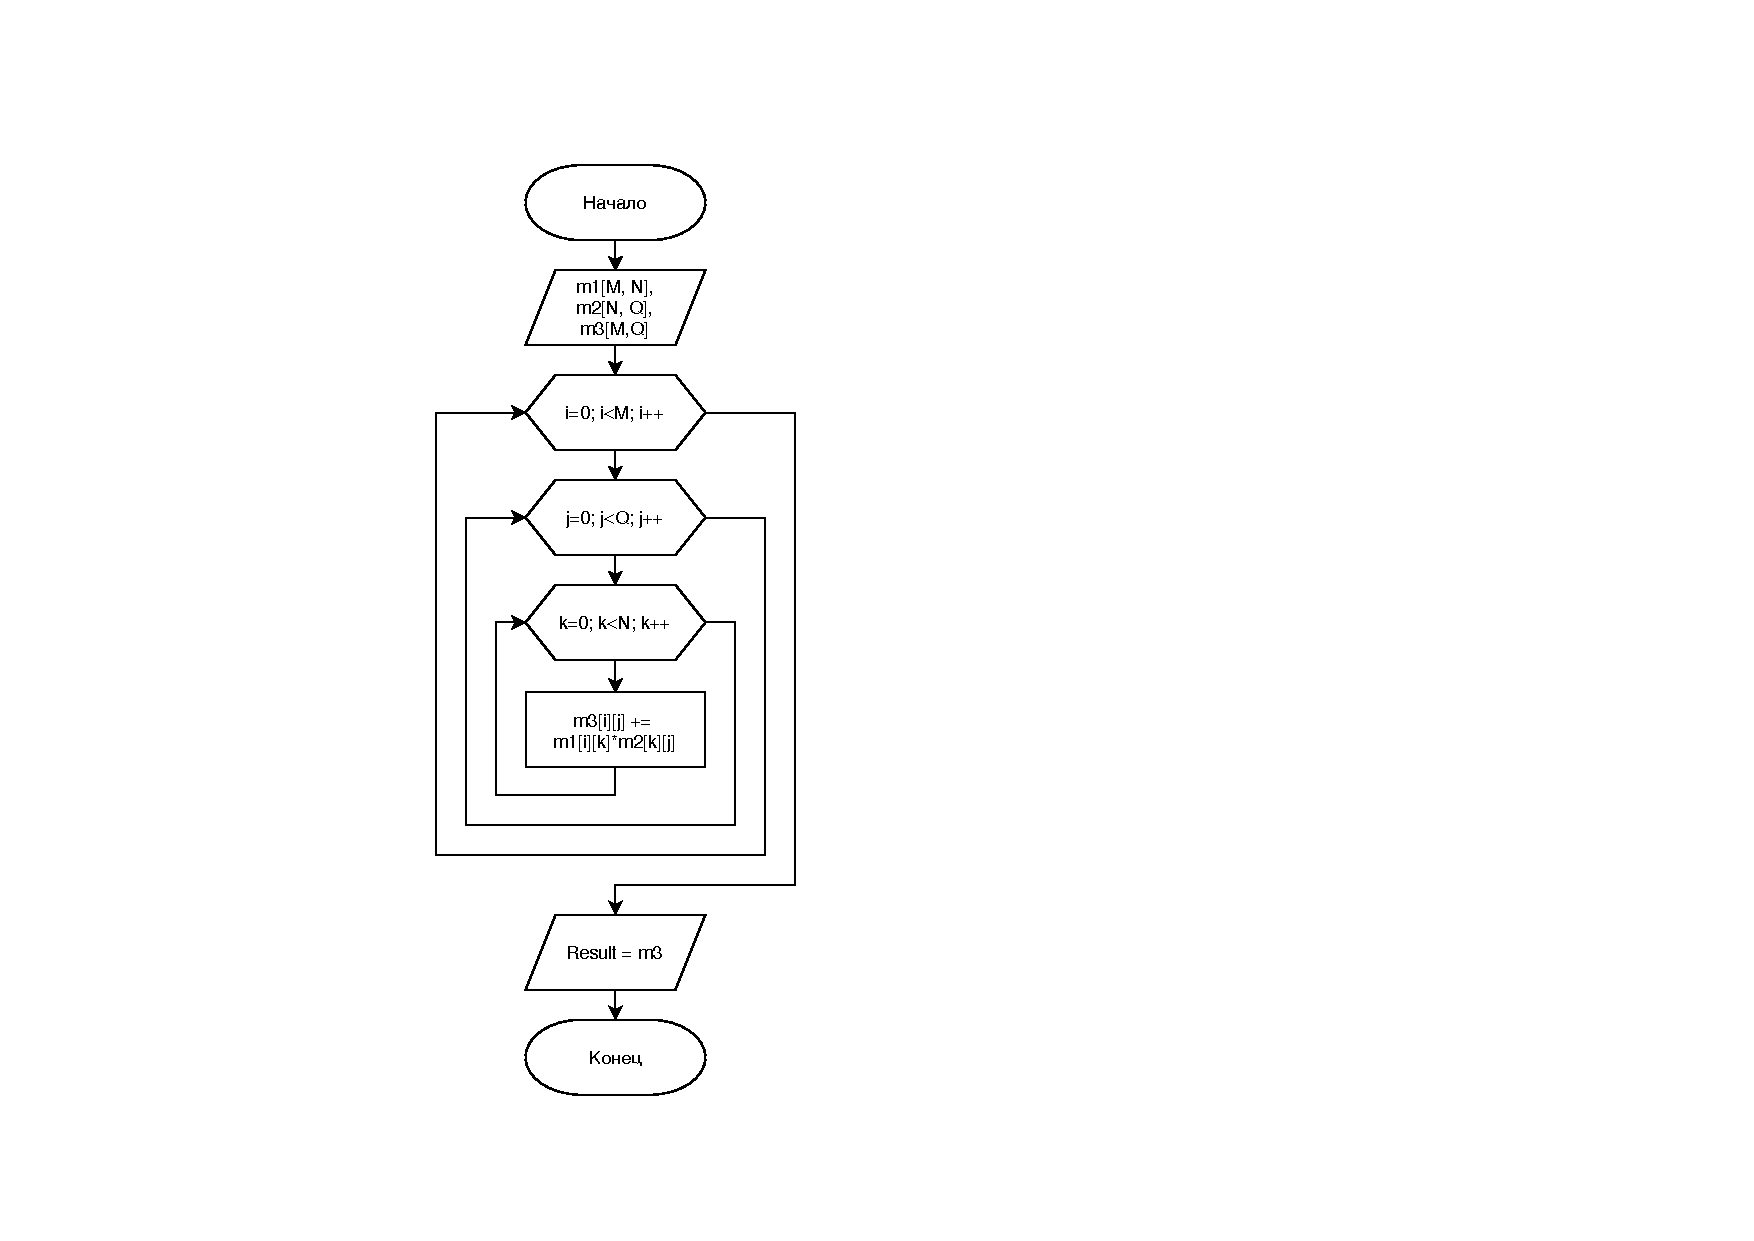
\includegraphics[scale=0.9]{schema_std.pdf}
            \caption{Схема стандартного алгоритма умножения матриц}
            \label{schema:standartDot}
    \end{figure}

    \begin{figure}[h!]
        \centering
            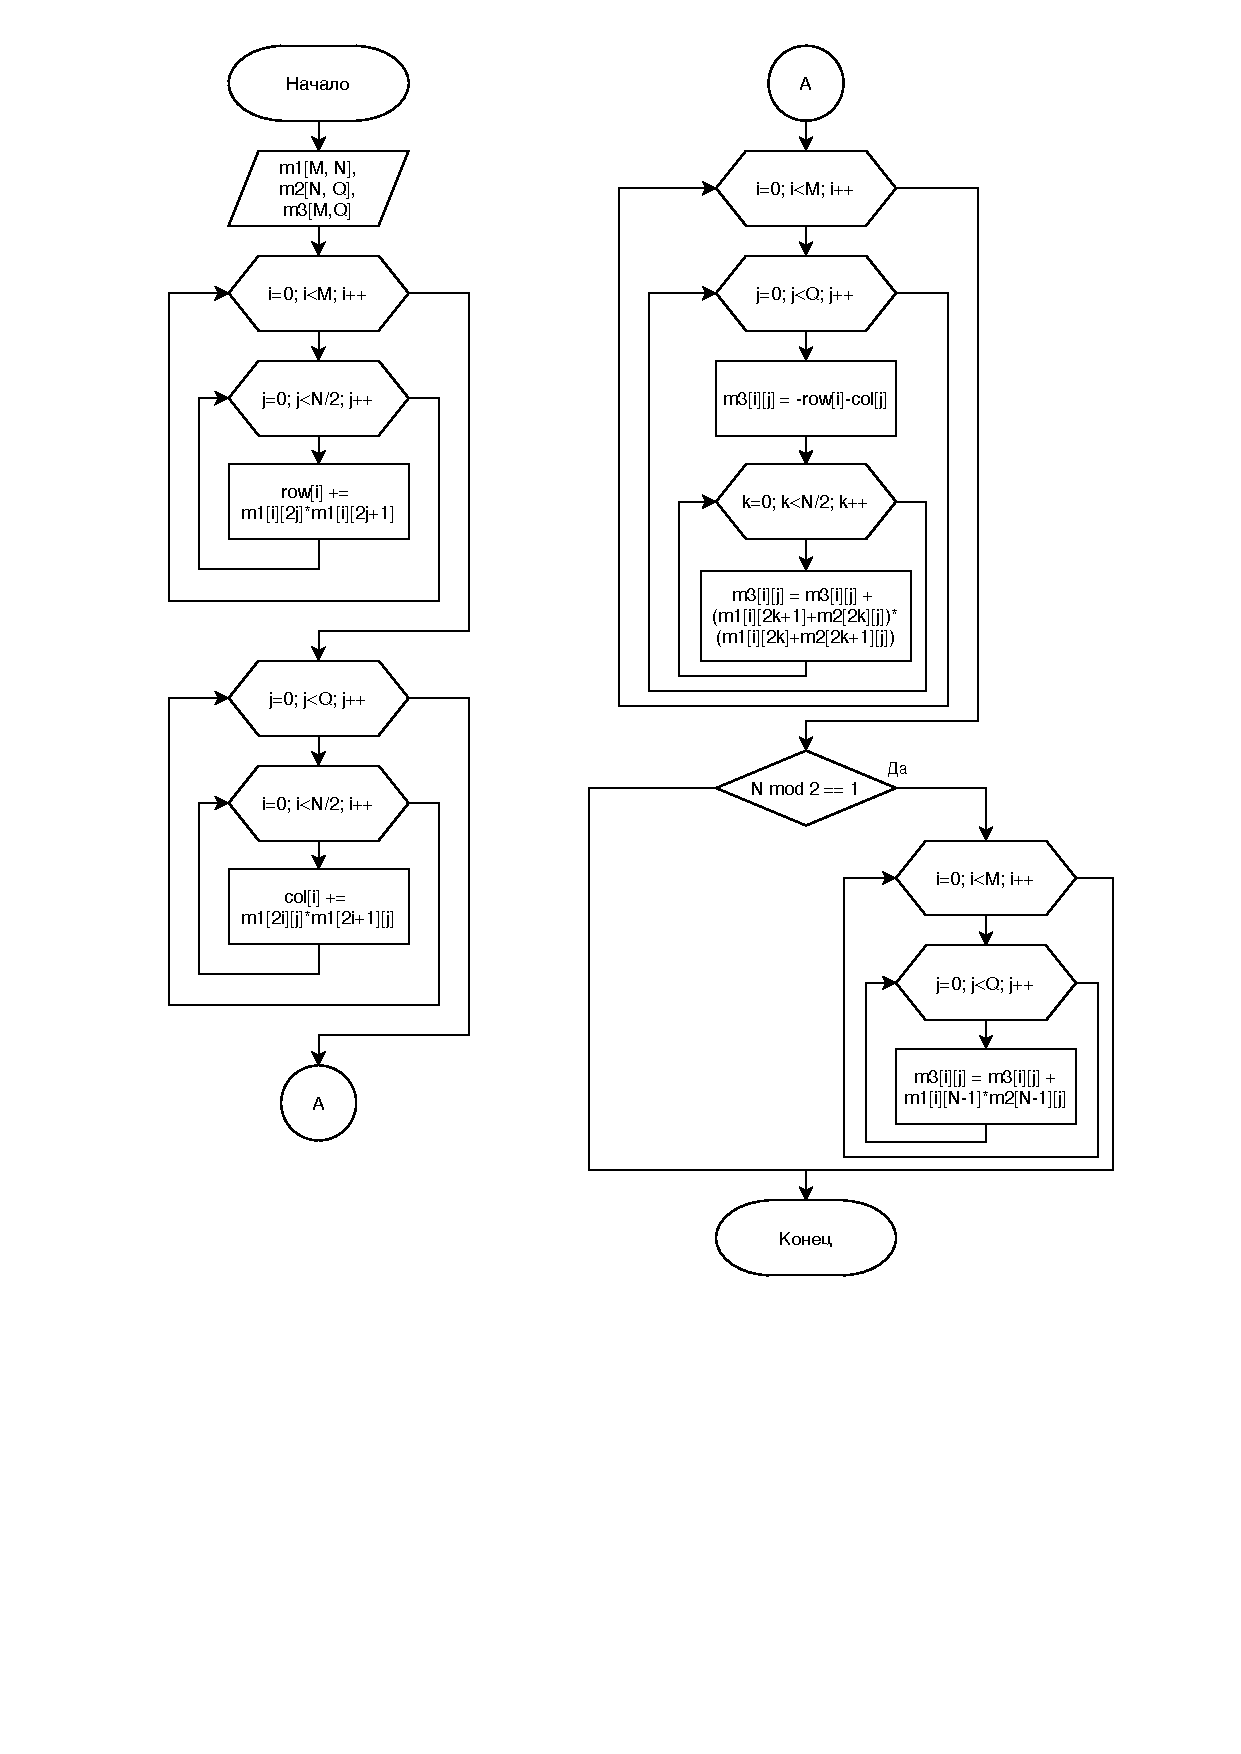
\includegraphics[scale=0.9]{schema_vin.pdf}
            \caption{Схема алгоритма умножения матриц методом Винограда}
            \label{schema:vinogradDot}
    \end{figure}

    \begin{figure}[h!]
        \centering
            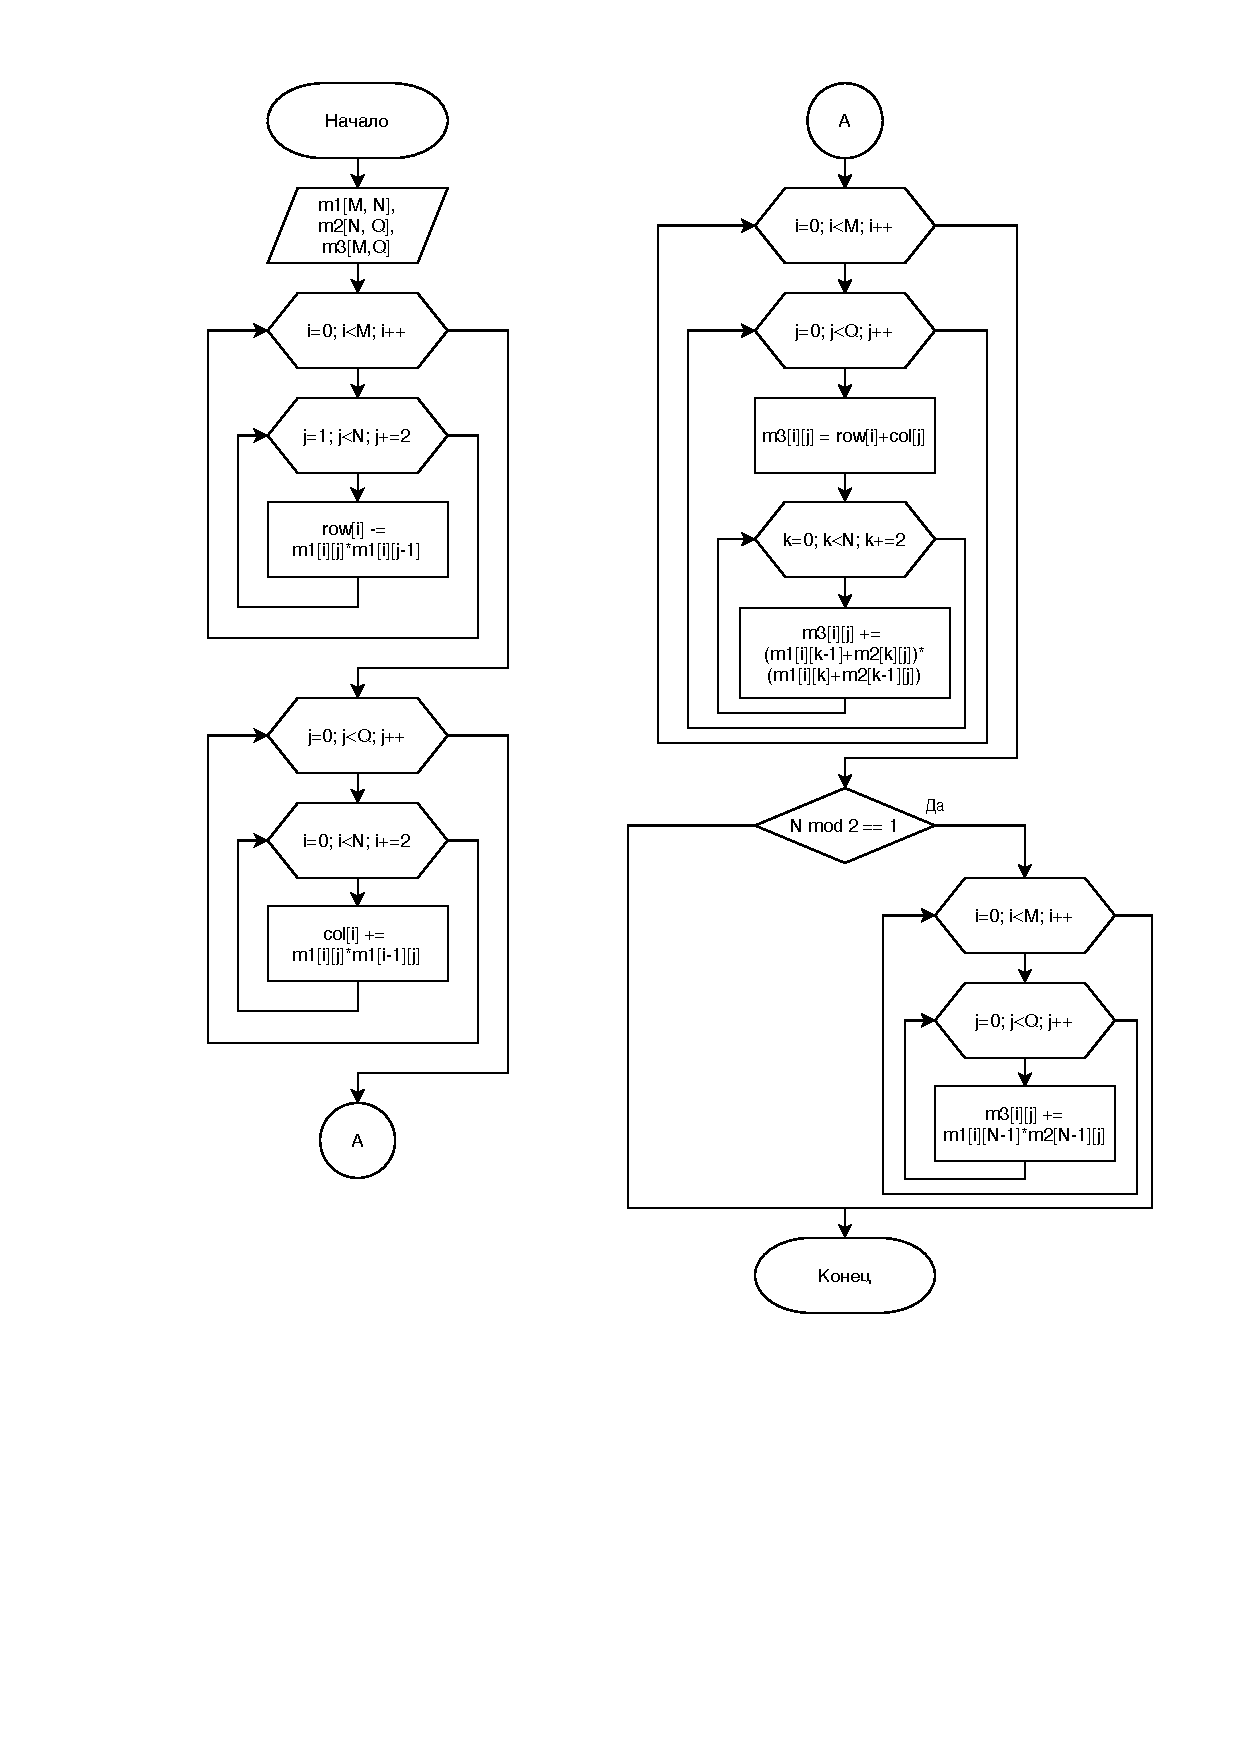
\includegraphics[scale=0.9]{schema_vinOpt.pdf}
            \caption{Схема оптимизированный алгоритм умножения матриц методом Винограда}
            \label{schema:vinogradDot:optimize}
    \end{figure}

    \section{Требования к функциональности ПО}
        В данной работе требуется обеспечить следующую минимальную функциональность консольного приложения:
        \begin{enumerate}
            \item возможность ввода двух матриц, на выходе результат произведения данных матриц? посчитанный трёмя алгоритмами;
            \item возможность вывода результатов замера процессорного времени работы реализаций каждого из алгоритмов. 
        \end{enumerate}

    \section{Тесты}
    Тестирование ПО будет проводиться методом чёрного ящика. Необходимо проверить работу системы 
    на тривиальных случаях (одна матрица единичная или нулевая) 
    и несколько нетривальных случаев.

\newpage